\documentclass{standalone}
\usepackage[T1]{fontenc}
\usepackage[utf8]{inputenc}
\usepackage{pgf,tikz}
\usepackage{pgfplots}
\pgfplotsset{compat=1.9}

\begin{document}

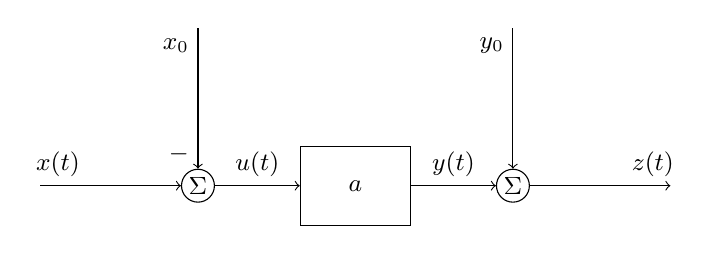
\begin{tikzpicture}[%
  node distance=2cm,
  block/.style={rectangle, draw, minimum width=14mm, minimum height=10mm},
  sum/.style={circle, thin, draw, inner sep=1pt},
  ]
  {\small 
    \node[coordinate] (input) {};
    \node[sum, right of=input,] (sum) {$\Sigma$};
    \node[block, right of=sum,] (sys) {$a$};
    \node[sum, right of=sys,] (sum2) {$\Sigma$};
    \node[coordinate, right of=sum2,] (output) {};
    \node[coordinate, above of=sum,] (oppoint) {};
    \node[coordinate, above of=sum2,] (oppoint2) {};
    \draw[->] (input) -- node[very near start, above] {$x(t)$} (sum);
    \draw[->] (oppoint) -- node[very near start, left] {$x_0$} node[pos=0.9, left] {$-$} (sum);
    \draw[->] (oppoint2) -- node[very near start, left] {$y_0$} node[pos=0.9, left] {} (sum2);
    \draw[->] (sum2) -- node[above, very near end] {$z(t)$} (output);
    \draw[->] (sum) -- node[above] {$u(t)$} (sys);
    \draw[->] (sys) -- node[above] {$y(t)$} (sum2);
}
\end{tikzpicture}
\end{document}
